\chapter{Grundlagen}
\label{sec:Grundlagen}
Leistungselektronik befasst sich mit der Umwandlung und Steuerung elektrischer Energie, um sie effizient in verschiedenen Formen für elektronische Geräte und Systeme nutzbar zu machen. Insbesondere die Entscheidung zwischen Wechsel- und Gleichstrom in den Übertragungs- und Verteilungsnetzen bleibt eine Debatte. Mit der Weiterentwicklung der Halbleitertechnik zeigt sich, dass die Gleichstromtechnik auch bei langen Übertragungsstrecken Vorteile gegenüber der verbreiteten Wechselstromtechnik hat. Um die Anforderungen und Zusammenhänge verstehen zu können, werden Details zur Elektrolyse, zu Stromrichtern und Komponenten sowie zur verwendeten Simulationsumgebung vorgestellt.
\section{Wasserstoff-Elektrolyse}
\label{sec:Elektrolyse}
Das Prinzip der \gls{AEL} ist, im Gegensatz zur neueren \gls{PEM} Elektrolyse, bereits seit langem bekannt und optimiert. Die \gls{AEL} benötigt in der Regel eine wässrige Kalilauge und kann durch Reihenschaltung der Zellen Wasserstoff und Sauerstoff unter erhöhtem Druck von z.~B. 30 bar bereitstellen. Die Entwicklung und insbesondere die Steigerung der Stromdichte und des Wirkungsgrades haben in den letzten Jahren keine großen Veränderungen gebracht. Der Spannungswirkungsgrad liegt zwischen 62 und 82 Prozent \cite{NOWH2}. Der Spannungswirkungsgrad bei der Elektrolyse von Wasserstoff bezieht sich auf das Verhältnis zwischen der tatsächlich benötigten elektrischen Spannung und der theoretisch erforderlichen Spannung, um Wasser in Wasserstoff und Sauerstoff zu spalten. Dieser kann im Verhältnis zur Stromdichte aufgetragen werden und bietet damit eine Übersicht über die Effizienz und Stromdichte, siehe Abbildung \ref{fig:ely-efficiency}. Die Stromdichte ist eine Vergleichsgröße für die benötigte Elektrodenfläche, den Platzbedarf und die benötigten Materialmengen.\\
Die \gls{PEM}-Elektrolyse bietet Vorteile durch erhöhte Stromdichte, bei größeren Anlagen spart dies unter anderem Platz, außerdem ist zu erwarten, dass Druckelektrolyse bis 100 bar möglich wird. Dies erhöht den Gesamtwirkungsgrad, da die Elektrolyseure den hohen Druck für die Lagerung oder den Transport generieren und somit Kompressoren eingespart werden können. Optimierungsbedarf besteht jedoch noch bei der Lebensdauer der Membranen und den benötigten Edelmetallen \cite{NOWH2}. \\
Die \gls{HTEL} nutzt die Vorteile höherer Temperaturen von oft über 500°C, die thermodynamische Vorteile für den elektrischen Wirkungsgrad bringen, jedoch hohe Anforderungen an die verwendeten Materialien stellen. Sie wird auch als Hochtemperatur-Wasserstoff-Festoxid-Elektrolysezelle (SOEC) bezeichnet. Der Name \glqq Festoxid\grqq bezieht sich auf die Art der Elektrolyten in der Zelle. In SOECs werden feste keramische Materialien als Elektrolyten verwendet, typischerweise aus Zirkonoxid (ZrO2) oder Yttrium-stabilisiertem Zirkonoxid (YSZ). Die Technologie der Festoxidelektrolyse befindet sich noch im Stadium der Grundlagenforschung im Labor. Da fast alle Festoxidzellen reversible Eigenschaften besitzen, ist das Interesse an ihnen besonders groß, da dies eine direkte Rückverstromung des Wasserstoffs ermöglicht. Allerdings sind auch hier noch Materialoptimierungen und Verbesserungen der Langzeiteigenschaften notwendig.\\
\begin{figure}
	\centering
	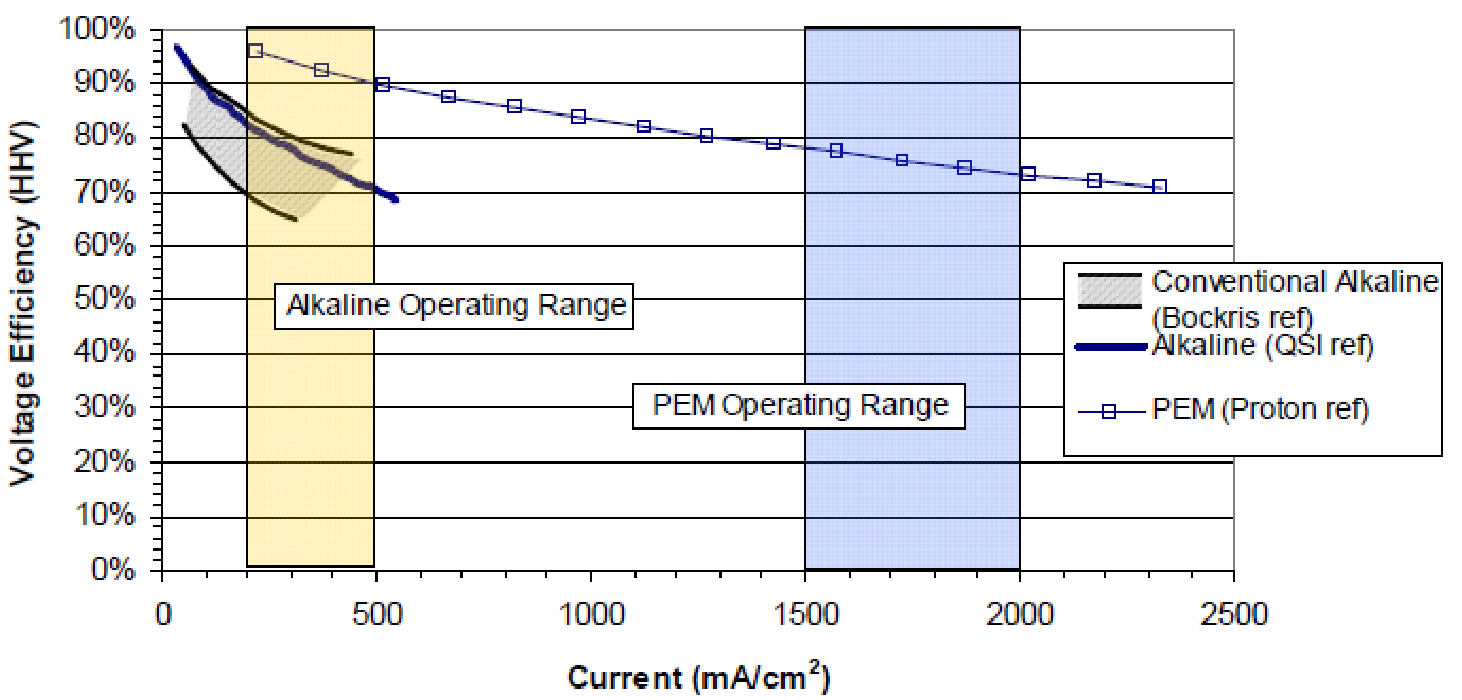
\includegraphics[width=0.9\linewidth]{content/Grafiken/Ely-Efficiency}
	\caption{Elektrolyseur Spannungseffizienz \cite{NOWH2}}
	\label{fig:ely-efficiency}
\end{figure}
\section{Stromrichter}
\label{sec:Stromrichter}
Allgemein kann jede Schaltung zur Strom- und Spannungsversorgung als Stromrichter bezeichnet werden, wobei zwischen AC- und DC-Varianten unterschieden wird. Weiterhin kann bei Netzanwendungen zwischen geregelt, netzgeführt und ungesteuert unterschieden werden, sowie die Implementierung einer \gls{PFC} betrachtet werden \cite{Schroder.2018}. Leistungshalbleiter und induktive Komponenten sind für den Aufbau von Stromrichterschaltungen unerlässlich. 
		\subsection{Leistungshalbleiter}
		Halbleiter sind im einfachsten Fall Bauelemente mit einem PN-Übergang; können sie größere Leistungen schalten, werden sie als Leistungshalbleiter bezeichnet. Dabei sind für die verwendete Topologie neben der klassischen Diode vor allem \gls{MOSFET} relevant. Diese verdrängen derzeit in der Leistungselektronik häufig den verbreiteten \gls{IGBT} aufgrund der preiswerter gewordenen Variante aus Siliziumkarbid \cite{SiCTrend}. Die Vorteile dieser neuen Technologie liegen in der Ermöglichung höherer Schaltfrequenzen, wodurch wiederum die in den induktiven Bauelementen zu speichernde Energie reduziert und somit Kosten eingespart werden können.\\
		Die heute industriell eingesetzten Halbleitermodule für leiterplattenmontierte Umrichter können Ströme von maximal 200 A führen. Für höhere Ströme müssen die Halbleiter parallel geschaltet werden, was den Schaltungsaufwand aufgrund der aufwendigen Realisierung des symmetrischen Schaltens erhöht. Um die Vorteile der \gls{SiC}-Halbleiter bei hohen Schaltfrequenzen nutzen zu können, werden nur Module mit geringer Induktivität betrachtet, so dass die Wahl auf Module mit Einpresskontakten fällt. Dies reduziert die Streuinduktivität des Moduls und der Verbindung zur Leiterplatte um bis zu einem Faktor 4 gegenüber dem von Infineon verwendeten EasyPack mit 62~mm Modulen \cite{IFAGFF2} \cite{IFAGFF2-62mm}. \\
		Zur Auswahl der am besten geeigneten Halbleiter werden unter anderem Schaltungssimulationen eingesetzt, diese erfordern eine Nachbildung der Halbleiter. Um die Modelle der Leistungshalbleiter zu erstellen und ggf. vorhandene Modelle zu validieren, können Messungen im \gls{DPT} durchgeführt werden. Ein Beispiel für die in \gls{PLECS} implementierten Ausschaltverluste eines Halbleiters zeigt Abb. \ref{fig:plecsff2thermalmodel}. Es ist zu erkennen, dass die Punkte nur für den Betriebspunkt von 600 Volt zur Verfügung stehen, für andere Betriebsbereiche muss das Verhalten approximiert werden. Außerdem ist der \gls{RGV} nur für einen begrenzten Bereich dargestellt und die \gls{VGSS} nur auf einen Wert beschränkt. Dies kann in der späteren Anwendung zu deutlichen Abweichungen führen. 
		\begin{figure}
			\centering
			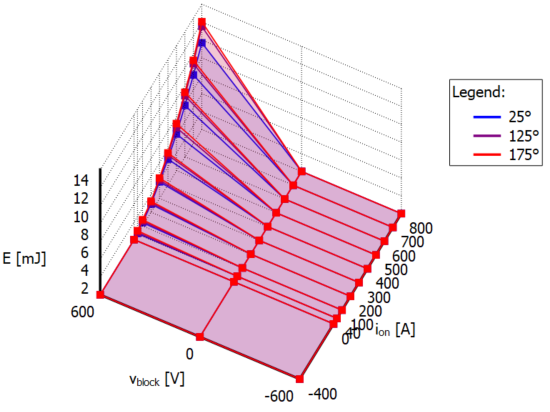
\includegraphics[width=0.7\linewidth]{content/Grafiken/PLECS_FF2ThermalModel}
			\caption{Darstellung der in PLECS implementierten Ausschaltverluste \cite{IFAGFF2}}
			\label{fig:plecsff2thermalmodel}
		\end{figure}
		
		\subsection{Induktive Komponenten}
		Induktive Bauelemente sind in der Regel Spulen und Transformatoren, die zur Speicherung und Übertragung von Energie dienen. Transformatoren bieten zusätzlich die Möglichkeit der galvanischen Entkopplung von Stromkreisen. 
		Für die Dimensionierung von Induktivitäten wird das Delta des Stromes in der Spule, der sogenannte Stromrippel, benötigt. Dieser Strom wird hier mit 30 Prozent des \gls{I^} ausgelegt. Für Drehstromsysteme kann der Rippelstrom nach der Formel \ref{eq:DeltaI} ermittelt werden. Dabei sind \gls{S} und \gls{Ull} die Spannungen zwischen den Außenleitern. \cite{Boge.2007}.\\
		\begin{equation}
			\label{eq:DeltaI}
			\hat{I} = 0,3 \cdot \dfrac{\sqrt{2} \cdot S}{\sqrt{3} \cdot U_{LL}}
		\end{equation}
		Außerdem kann über die gespeicherte \gls{WL} eine Aussage über die Größe und damit indirekt über die Kosten und den Platzbedarf getroffen werden. Die Energie \gls{WL} kann mit der Formel \ref{eq:WL} berechnet werden. Dazu wird der Wert der Induktivität und der Strom benötigt \cite{Boge.2007}.
		\begin{equation}
			\label{eq:WL}
			W_{L} =\dfrac{1}{2}\cdot L\cdot \hat{I}^{2}
		\end{equation}
		
		\subsection{Gleichrichter}
		\label{sec:Rec}
		Ein Gleichrichter wird genutzt, um aus einer Wechselspannung eine Gleichspannung zu erzeugen. Die einfachste Form ist der Diodengleichrichter. Dieser kann für einphasige Wechselspannung durch eine einzelne Diode realisiert werden. Allerdings würde so nur die halbe Periode des Sinus am Ausgang zur Verfügung stehen, da die Diode nur während der positiven Halbwelle leitet. Dies kann durch die Ergänzung eines Brückengleichrichters mit vier Dioden für einphasige Anwendungen und sechs Dioden für dreiphasige Anwendungen optimiert werden. Der dreiphasige Diodengleichrichter findet sich in Abbildung \ref{fig:B6DiodRect}. 
		\begin{figure}[H]
			\centering
			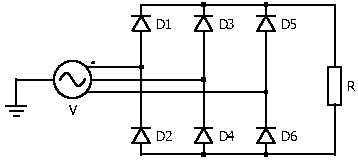
\includegraphics[width=0.8\linewidth]{content/Grafiken/Plecs_Diodengleichrichter.pdf}
			\caption{Diodengleichrichter für dreiphasige Anwendungen}
			\label{fig:B6DiodRect}
		\end{figure}
		Der Diodengleichrichter ist jedoch nur bedingt für einen gewünschten Stromverlauf geeignet. In Abbildung \ref{fig:B6DiodRectI} ist der Netzspannungs und Stromverlauf des Diodengleichrichter dargestellt. Der Stromverlauf zeigt starke Sprünge und der gewünschte sinusförmige Verlauf ist nur schwer erkennbar, dies kann durch Ergänzung von Kondensatoren und Spulen zur Filterung teilweise korrigiert werden. Dies wäre jedoch nur für einen festen Betriebspunkt möglich. Außerdem ist es mit dieser Schaltung nicht möglich, die Ausgangsspannung oder den Strom zu variieren.
		\begin{figure}
			\centering
			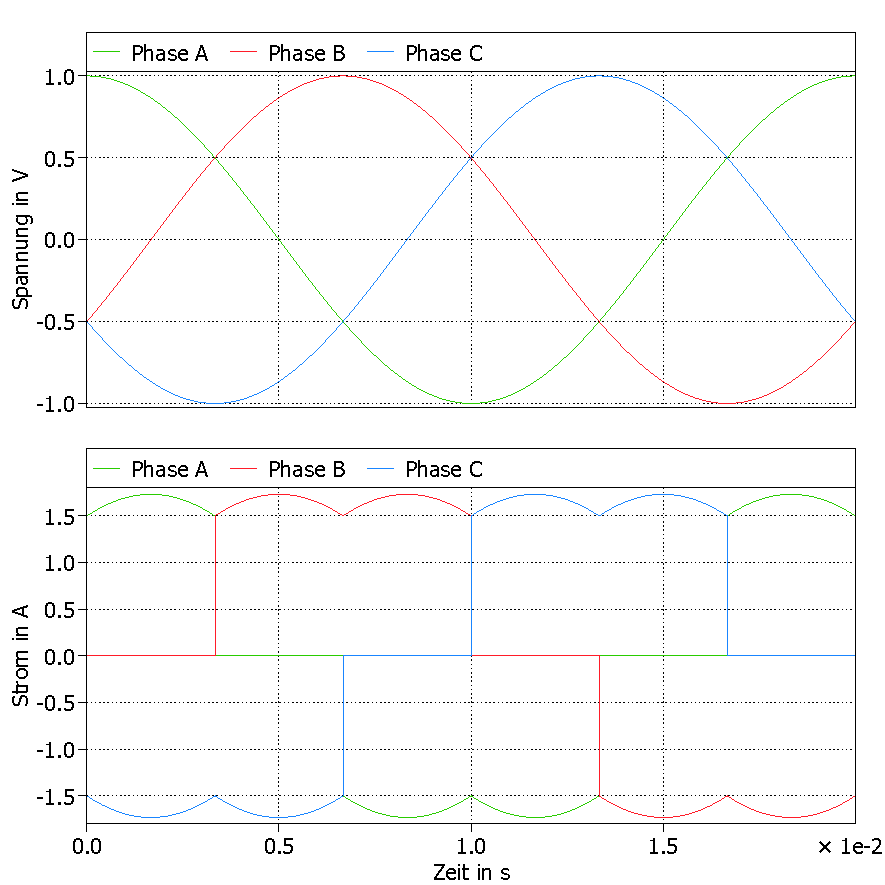
\includegraphics[width=0.8\linewidth]{content/Grafiken/B6-Diodengleichrichter-Eingangsverlauf}
			\caption{Strom und Spannungsverlauf des Dreiphasigen Diodengleichrichters }
			\label{fig:B6DiodRectI}
		\end{figure}
		Eine Möglichkeit zur Regelung der Aus- oder Eingangsspannung bieten Thyristorgleichrichter, diese lassen sich in großen Leistungsklassen zentral aufbauen, bieten jedoch oft nicht die nötige Flexibilität. 
		Mit thyristorbasierten Schaltungen können große Leistungen effizient umgesetzt werden, allerdings führen sie zu deutlichen Verzerrungen im Stromverlauf und zu einem schlechteren Leistungsfaktor. Sie erfordern daher passive oder aktive Filter, die die Systemkosten erhöhen \cite{HydrogenElectronicTopologies}. Die Parallelisierung mit phasenversetzter Ansteuerung bietet deutliche Vorteile durch geringere Verzerrung und damit weniger Filteraufwand. Bei versetzter Ansteuerung überlagern sich die Eingangsströme zu einem weniger verzerrtem Stromverlauf.\\
		Alternativ werden \gls{AFE} Gleichrichter eingesetzt, die wesentlich geringere Verzerrungen und mehr Freiheit bei der Regelung des Eingangsstroms bieten. Die Filter sind wesentlich kleiner und auf eine Blindleistungskompensation kann in diesem Fall verzichtet werden \cite{HydrogenElectronicTopologies}. Bei \gls{AFE} Gleichrichtern werden Schaltungen zusammengefasst, die aktiv gesteuert werden und dadurch eine bessere Leistung und Kontrolle des Stromflusses ermöglichen. Diese benötigen \gls{IGBT}- oder \gls{MOSFET}-Schalter für die aktive Steuerung. Parameter, die bei diesen Systemen aktiv beeinflusst werden können, sind die Leistungsfaktorkorrektur, ein regelbarer Energiefluss (manchmal sogar bidirektional) und Oberschwingungen, die reduziert werden können \cite{HydrogenElectronicTopologies}.
		\subsection{DC-DC Wandler} \label{sec:Buck}
		Der Hochsetzsteller (Boost-Converter) und der Tiefsetzsteller (Buck-Converter) sind grundlegende Topologien, die im Wesentlichen aus zwei Halbleitern und einer Induktivität bestehen. In Abb. \ref{fig:buck} ist die Schaltung eines Tiefsetzstellers dargestellt. Über das \gls{D} des Schalters kann die \gls{Ua} eingestellt werden, wobei die Parameter \gls{Ue}, Lastimpedanz sowie der Wert der Induktivität relevant sind. Die Ausgangsspannung kann für den kontinuierlichen Betrieb über die Beziehung $U_{a}=D\cdot U_{e} $ berechnet werden \cite{schmidtwalter}.
		\begin{figure} [t]
			\centering
			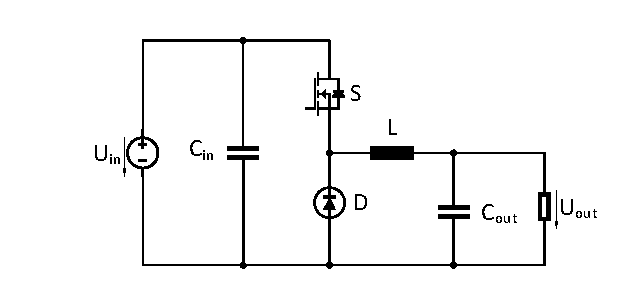
\includegraphics[width=0.9\linewidth]{content/Grafiken/Buck}
			\caption[Tiefsetzsteller]{Tiefsetzsteller}
			\label{fig:buck}
		\end{figure}
		Die Speicherdrossel des Tiefsetzstellers kann nach der Formel \ref{eq:BuckL} ausgelegt werden, wobei der gewünschte Stromrippel $\Delta I $ in der Drossel auf maximal 30~\% des \gls{Ia} festgelegt wird \cite{schmidtwalter}. Ein Stromrippel von 30 \% erweist sich als guter Kompromiss zwischen dem Induktivitätswert und der Größe der Rippelamplitude. Durch steile Amplituden können Störungen durch elektromagnetische Felder verursacht werden und der Filterbedarf am Ein- und Ausgang steigt \cite{AnalogInductor} \cite{TIBuck}.
		\begin{equation}
			\label{eq:BuckL}
			L=\dfrac{U_{e,max}-U_{a}}{f\cdot \Delta I}\cdot D = \dfrac{U_{e,max}-U_{a}}{f\cdot 0,3 \cdot I_{a}}\cdot \dfrac{U_{a}}{U_{e,max}}
		\end{equation}
		Wird die Eingangsspannung durch einen dreiphasigen Diodengleichrichter, wie in Abb. \ref{fig:B6DiodRect} dargestellt,  implementiert, so kann die Eingangsspannung mit $U_{LL} \cdot \sqrt{2}$ berechnet werden. Die Spannung zwischen den Außenleitern \gls{Ull} wird als \gls{RMS} Wert angegeben, daraus kann über den Faktor $\sqrt{2}$ der Spitzenwert bestimmt werden. Daraus ergibt sich die Formel \ref{eq:BuckLB6} bezogen auf die Phasenspannungen. \\
		\begin{equation}
			\label{eq:BuckLB6}
			L=\dfrac{U_{LL} \cdot \sqrt{2}-U_{a}}{f\cdot 0,3 \cdot I_{a}}\cdot \dfrac{U_{a}}{U_{LL} \cdot \sqrt{2}}
		\end{equation}
		Zusätzlich besteht die Option des Interleavings, das die Verflechtung von Schaltungen impliziert, also die Integration mehrerer Schaltungen in einer einzigen Einheit, wie in der Abbildung \ref{fig:buckinterleaved} dargestellt. Die Taktung der Halbleiter wird versetzt ausgeführt und benötigt eine gekoppelte Steuerung. Dadurch können einerseits die Drosseln besser ausgenutzt und andererseits die Welligkeit des Ausgangsstroms halbiert werden. 
		\begin{figure}
			\centering
			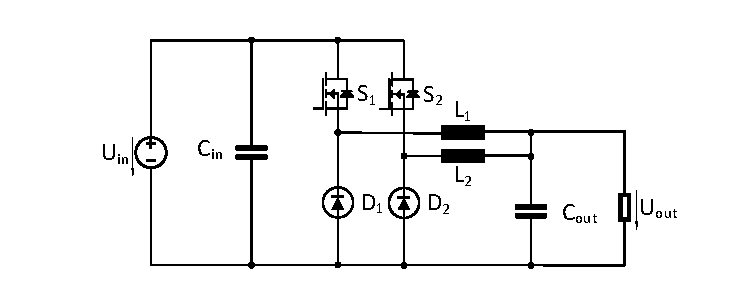
\includegraphics[width=0.7\linewidth]{content/Grafiken/Buck_interleaved}
			\caption{Tiefsetzsteller mit Interleaving}
			\label{fig:buckinterleaved}
		\end{figure}
		
		

		\subsection{Power Factor Correction (PFC)}
		Die \gls{PFC} ist eine notwendige Maßnahme, um den Blindleistungsanteil im Netz zu reduzieren und ist daher in heutigen Geräten standardmäßig implementiert. Ein Beispiel aus der Industrie, bei dem eine einfache Blindleistungskompensation bereits realisiert wurde, sind Leuchten mit Halogenlampen. Diese waren mit einem Transformator zur Erzeugung der notwendigen Spannung ausgestattet, der jedoch Blindleistung verursachte, was durch einfaches Hinzufügen eines Kondensators optimiert werden konnte. \\
		In herkömmlichen Gleichrichtersystemen werden getrennte Einheiten, bestehend aus einer dreiphasigen PFC-Gleichrichterschaltung und einem Gleichspannungswandler (DC/DC-Buck-Wandler), eingesetzt, um die Anforderungen zu erfüllen. Die Regelung der beiden Wandlerstufen erfolgt in der Regel entkoppelt, wobei der Gleichrichter sinusförmige Netzströme aufnimmt und der nachfolgende DC/DC-Wandler die Spannung an die erforderliche Ausgangsspannung anpasst. Das Streben nach kompakten und leichten Systemen erfordert hohe Schaltfrequenzen, die jedoch zu erhöhten Schaltverlusten und verringertem Wandlerwirkungsgrad führen können. Um dieses Problem zu lösen, können fortgeschrittene Modulationstechniken wie die Einfügung der dritten Harmonischen und Raumzeigermodulation eingesetzt werden. Alternativ kann die diskontinuierliche Pulsweitenmodulation (DPWM) als Methode zur Reduzierung der Schaltverluste in dreiphasigen PFC-Gleichrichtern eingesetzt werden, um sinusförmige Eingangsströme und eine konstante Gleichspannung zu gewährleisten. Im Gegensatz dazu müssen einstufige Umrichtersysteme beide Anforderungen gleichzeitig erfüllen, während zweistufige Systeme eine konstante Ausgangsspannung trotz niederfrequenter Spannungsschwankungen im Gleichspannungszwischennetz gewährleisten können.			
		
				
			



\section{Simulationssoftware}
	Um die Machbarkeit von Topologien bewerten und untersuchen zu können, ist es notwendig, diese in einer Gesamtsimulation zu betrachten. Dies ermöglicht es, die Funktionalität und den Einfluss der Parameter im direkten Zusammenspiel zu untersuchen. Insbesondere das Verhalten für Systemdienstleistungen, wie die Phasenverschiebung und die dadurch beeinflusste Verteilung der Verlustleistungen, soll als Entscheidungsgrundlage dienen.\\
	Es wird die Version R2022a von Matlab mit Simulink Version 10.5 und Plecs Version 4.6.8 verwendet.  

	\subsection{PLECS}
	Die Software \gls{PLECS} der Firma PLEXIM wird als Integration in MATLAB mit Simulink verwendet.  Sie ermöglicht die Modellierung von Schaltungen unter Berücksichtigung des thermischen Verhaltens durch elektrische Verlustleistungsmodelle. Dazu wird die Energie im Schaltvorgang sowie im durchgeschalteten Zustand in der Schaltung berücksichtigt. Dies ermöglicht die Betrachtung der Verlustleistung innerhalb des Halbleiters und damit den Aufwand für die Kühlung und eine Abschätzung des Wirkungsgrades der Schaltung. Ein Beispiel der Funktionen ist in Abb. \ref{fig:plecsbuck} zu sehen, die thermische Kette muss aus Datenblättern o.~ä. der Kühlkörper bekannt sein. Um die Leitverluste zu bestimmen, werden periodische Mittelwerte der Verlustleistung im Halbleiter gebildet, um eine Aussage über die gesamte Periode zu bilden. Für die Schaltverluste werden die periodischen Impulsmittelwerte gebildet, da die Schaltvorgänge im Modell nur sehr steile Impulse sind. Für Halbleiter werden thermische Modelle benötigt, die ebenfalls aus Datenblättern erstellt oder vom Hersteller zur Verfügung gestellt werden können. Allerdings gibt es nicht für alle Halbleiter ausreichende Informationen und die tatsächliche Verlustleistung hängt von vielen Parametern ab. Daher ist es oft notwendig, eigene Messungen durchzuführen, um die spätere Anwendung bestmöglich simulieren zu können. In den verwendeten Modellen der Leistungshalbleiter wird die Thermische kette bereits im Modell berücksichtigt und muss daher nicht als externer Block wie in Abbildung \ref{fig:plecsbuck} berücksichtigt werden. Außerdem werden die zeitlichen Konstanten in den Modellen verringert, um schneller einen eingeschwungenen Zustand zu erreichen. \\
	
	\begin{figure}
		\centering
		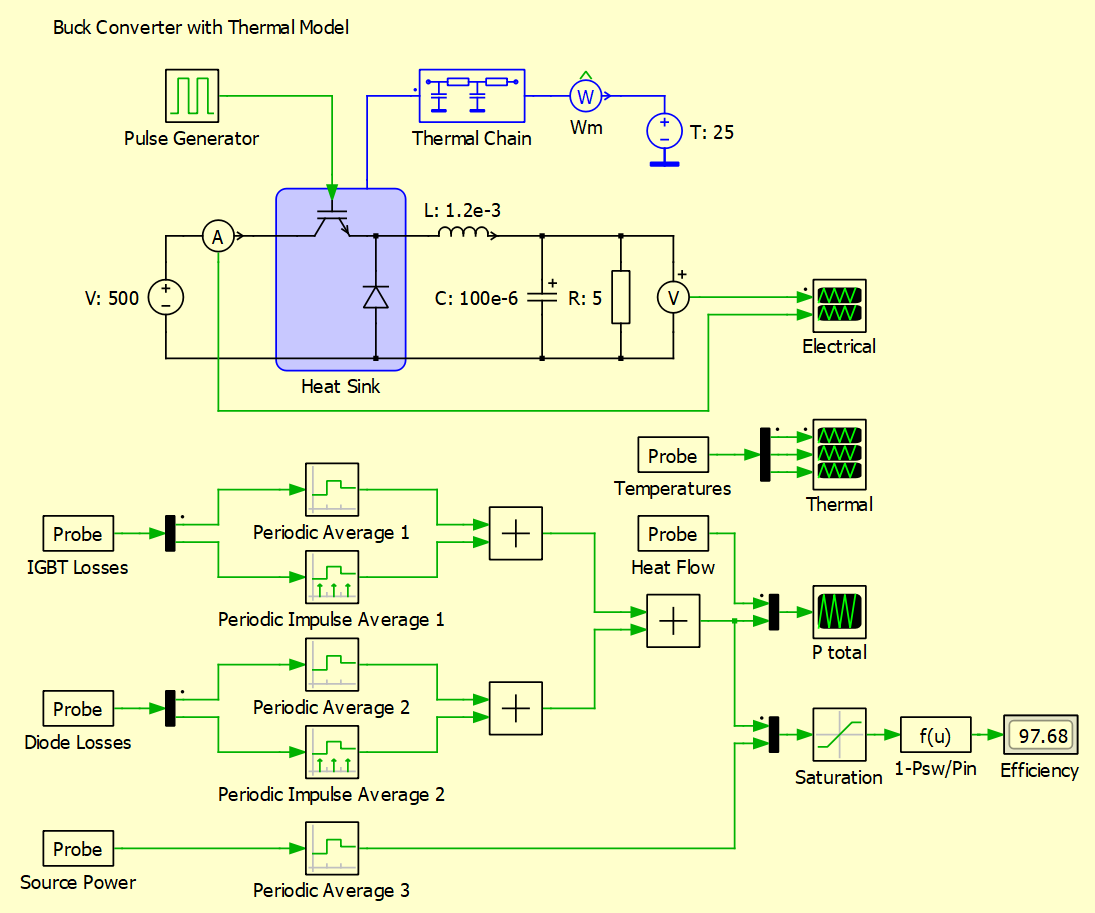
\includegraphics[width=1\linewidth]{content/Grafiken/PLECS_Buck}
		\caption[Tiefsetzsteller mit Effizienzbestimmung]{Tiefsetzsteller mit Effizienzbestimmung}
		\label{fig:plecsbuck}
	\end{figure}
	